\section{Introduction}

Empirical scaling laws for language model pretraining~\citep{kaplan_scale, hoffmann2022training, openai2023gpt4, openai2024openai, geminiteam2023gemini, henighan2020scaling, clark2022unified, yun2024toward, ludziejewski2024scaling} have demonstrated that proportionally increasing model capacity, along with data and total compute budget, consistently decreases pretraining loss (i.e., perplexity), improves downstream task performance~\citep{devlin_acl_2019_bert, brown_neurips2020_few_shot, srivastava2023beyond} and unlocks emergent capabilities~\citep{wei2022emergent}.

A recurring notion in these studies is that model capacity is well quantified by the total number of model parameters.
However, the number of parameters is not the only means to increase model capacity. \emph{Compute per example (i.e., a fixed-sized input)}, measured in FLoating OPerations (\flops), also plays a significant role~\citep{clark2022unified}. 
In fact, several mechanisms~\citep{shazeer2017,dehghani2018universal,wei2022chain_cot, goyal2024think_pause,Csordas2024MoEUTMU} allow for independent variation of the number of parameters or \flops per example within a model. 
For instance, Sparse Mixture-of-Experts (MoE) models~\citep{shazeer2017} introduce ``FLOP-free parameters'' by leveraging sparsity, where only a subset of expert modules is activated for each input.

\begin{figure*}[!t]
    \centering
    \subfigure[IsoFLOP surface over sparsity and total parameters]{
        \label{fig:iso_surface_total}
        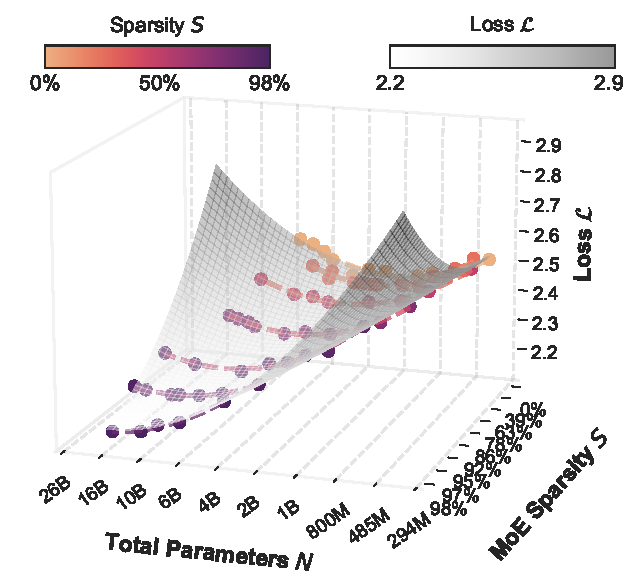
\includegraphics[width=0.45\textwidth]{plots/3d_suface_fit_total_params.pdf}
    }
    \quad %\hfill
    \subfigure[IsoFLOP surface over sparsity and active parameters]{
        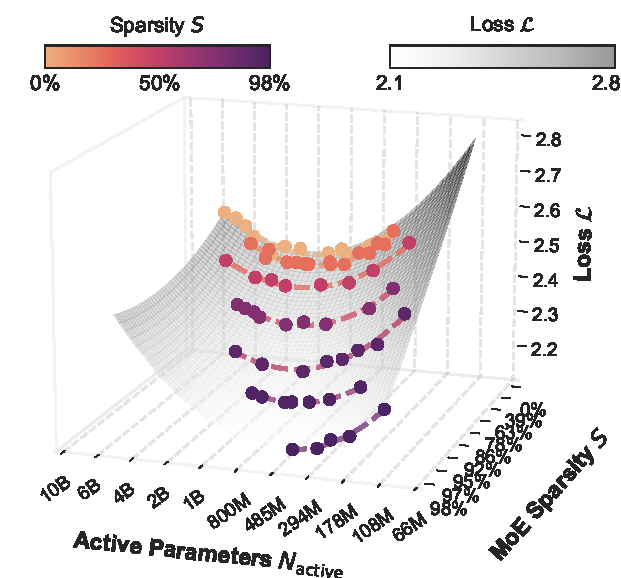
\includegraphics[width=0.45\textwidth]{plots/3d_suface_fit_active_params.pdf}
        \label{fig:iso_surface_active}
    }
    \caption{\textbf{IsoFLOP surface over observed pretraining loss $\mathbf{L}$, model size (in terms of total $\mathbf{N}$ and active parameters $\mathbf{N_a}$), and sparsity $\mathbf{S}$.} We fit a polynomial function mapping $\mathbf{N}$ (or $\mathbf{N_a}$), $\mathbf{S}$, and their interaction to $\mathbf{L}$, using empirical data. For both fits the MSE loss for predicting loss on a held out set is $0.0001$. These results indicate that for a fixed compute budget, increasing model sparsity leads to a reduction in pretraining loss. When considering optimal model size, we observe opposite trends for total parameters ($\mathbf{N}$) (Figure a) versus active parameters ($\mathbf{N_a}$) (Figure b). (See \Cref{fig:additional_surfaces} in \Cref{app:n_s_d_interaction} for results with different total compute budgets $C$.)}
    \label{fig:iso_surface}
\end{figure*}


When studying scaling laws for specific classes of models, e.g., vanilla transformers, the total number of parameters can serve as a reasonable relative estimator of \flops per example. 
Therefore, using the number of parameters as a measure of model capacity in scaling law studies is appropriate. 
In scenarios or for architectures where the number of parameters and \flops per example are not directly linked, it is essential to jointly consider the effects of these variables on scaling model capacity~\citep{clark2022unified}.
We therefore ask
\begin{center}
\emph{``Can we draw scaling laws for the optimal trade-off between\\parameter count and \flops per example?''} 
\end{center}
To address this question, we study sparse Mixture-of-Expert Transformers (\moes)~\citep{shazeer2017,lepikhin2021gshard,fedus_switch,zoph2022st,muennighoff2024olmoe} in the context of language modeling.
Existing scaling law studies for \moes, investigate the role of variables like number and granularity~\citep{ludziejewski2024scaling} of experts, underlying dense model size and inference compute in predicting the performance of the models under different conditions such as training or inference compute optimality~\citep{Du2021GLaMES,clark2022unified,yun2024toward,ludziejewski2024scaling}. In this paper, we focus on the interaction between \flops per example and total parameter count, and their impact on model performance in \moes, through a large-scale empirical study. 

 
We define sparsity as the ratio of inactive experts to the total number of experts, which controls the ratio of the total number of parameters to \flops per example in \moes. We evaluate loss and downstream metrics for different sparsities, model sizes, and compute budgets.
Through qualitative and quantitative analysis to derive scaling laws which disentangle total parameters vs \flops per example in \moes, we can estimate the optimal sparsity level under the setting where both total training \flops and total number of parameters are given and fixed. Generally, we find that:
\begin{itemize}

\item During pretraining, increasing a model’s capacity by adding more parameters yields greater benefits than increasing \flops per example. We observe that the size of compute-optimal models increases as we increase the training budget (measured in terms of total \flops) while the active number of parameters, hence \flops per example, decrease for compute-optimal models.

\item During inference, \flops per example seem to play a more important role\footnote{A relevant discussion here is the recent trend of increasing test-time compute, e.g., OpenAI o1 model~\citep{openai2024openai}, achieved by generating more tokens as a way for introducing parameter-free-FLOPs.}.
For many tasks, upstream performance is a good predictor of downstream performance and the relationship between upstream and downstream performance is not impacted by the sparsity level. However, on downstream tasks that presumably require more ``reasoning'', we observe that for models with the same perplexity on the pretraining data distribution, sparser models, i.e., models with fewer active parameters, perform worse. 
\end{itemize}


Our results, in line with findings from previous relevant studies~\citep{ludziejewski2024scaling,he2024mixture} on scaling laws for \moes, show increasing sparsity level leads to better performance and efficiency during pretraining. 
Considering the various methods to increase compute per example during inference adaptively conditioned on task or example complexity, we conclude that approaches like \moes, which reduce the unit compute cost (i.e., FLOPs per token) by increasing the sparsity level, hold significant promise given their potential to enhance efficiency in both pretraining and inference.
